\section{Motivation}
\label{sec:motivation}
As mentioned in section \ref{sec:intro}, the pros and cons are listed in the follwing Table \ref{table:regVsirreg}.
Regular prefetchers are good at prefetching regular patterns but inaccurate at irregular patterns. On the other hand, irregular prefetchers are good at prefetching irregular patterns but inefficient at regular patterns. Obviously, the advantage and disadvantage of these two kinds of prefetchers are complimentary.
%One straightforward idea is to identify regular patterns and irregular patterns during execution and apply corresponding prefetcher to issue prefetches.

\begin{table}[ht!]
\centering
\begin{tabular}{cccll}
\cline{1-3}
\multicolumn{1}{|c|}{}                     & \multicolumn{1}{c|}{Regular Access Pattern}             & \multicolumn{1}{c|}{Irregular Access Pattern}          &  &  \\ \cline{1-3}
\multicolumn{1}{|c|}{Regular Prefetcher}   & \multicolumn{1}{c|}{Accurate}              & \multicolumn{1}{c|}{{\color[HTML]{FE0000} Inaccurate}} &  &  \\ \cline{1-3}
\multicolumn{1}{|c|}{Irregular Prefetcher} & \multicolumn{1}{c|}{{\color[HTML]{FE0000} Inefficient}} & \multicolumn{1}{c|}{Accurate} &  &  \\ \cline{1-3}
\end{tabular}
\caption{Regular Vs. Irregular}
\label{table:regVsirreg}
\end{table}

  \subsection{Irregular Vs. Regular}
  \label{sec:irrVsre}
  Here we will show the performance graph of one regular benchmark and one irregular benchmark. In Fig.\ref{fig:regVsirreg}, \emph{libquantum} is a regular benchmark while \emph{omnetpp} is sort of an irregular benchmark. We can see that, though \emph{ISB} and \emph{BO} have similar accuracy but \emph{BO}'s coverage is better, so it has much more speedup than \emph{ISB}'s. That's why we call irregualr prefetchers are inefficient in detecting regular patterns. On the other hand, \emph{ISB} is much better than BO for benchmark \emph{omnetpp}. \emph{BO} even causes negative coverage because of huge cache pollution. This example shows that choosing a right prefetcher for one kind of access pattern is crucial to improve performance.
  \begin{figure}[ht!]
	  \centering
	  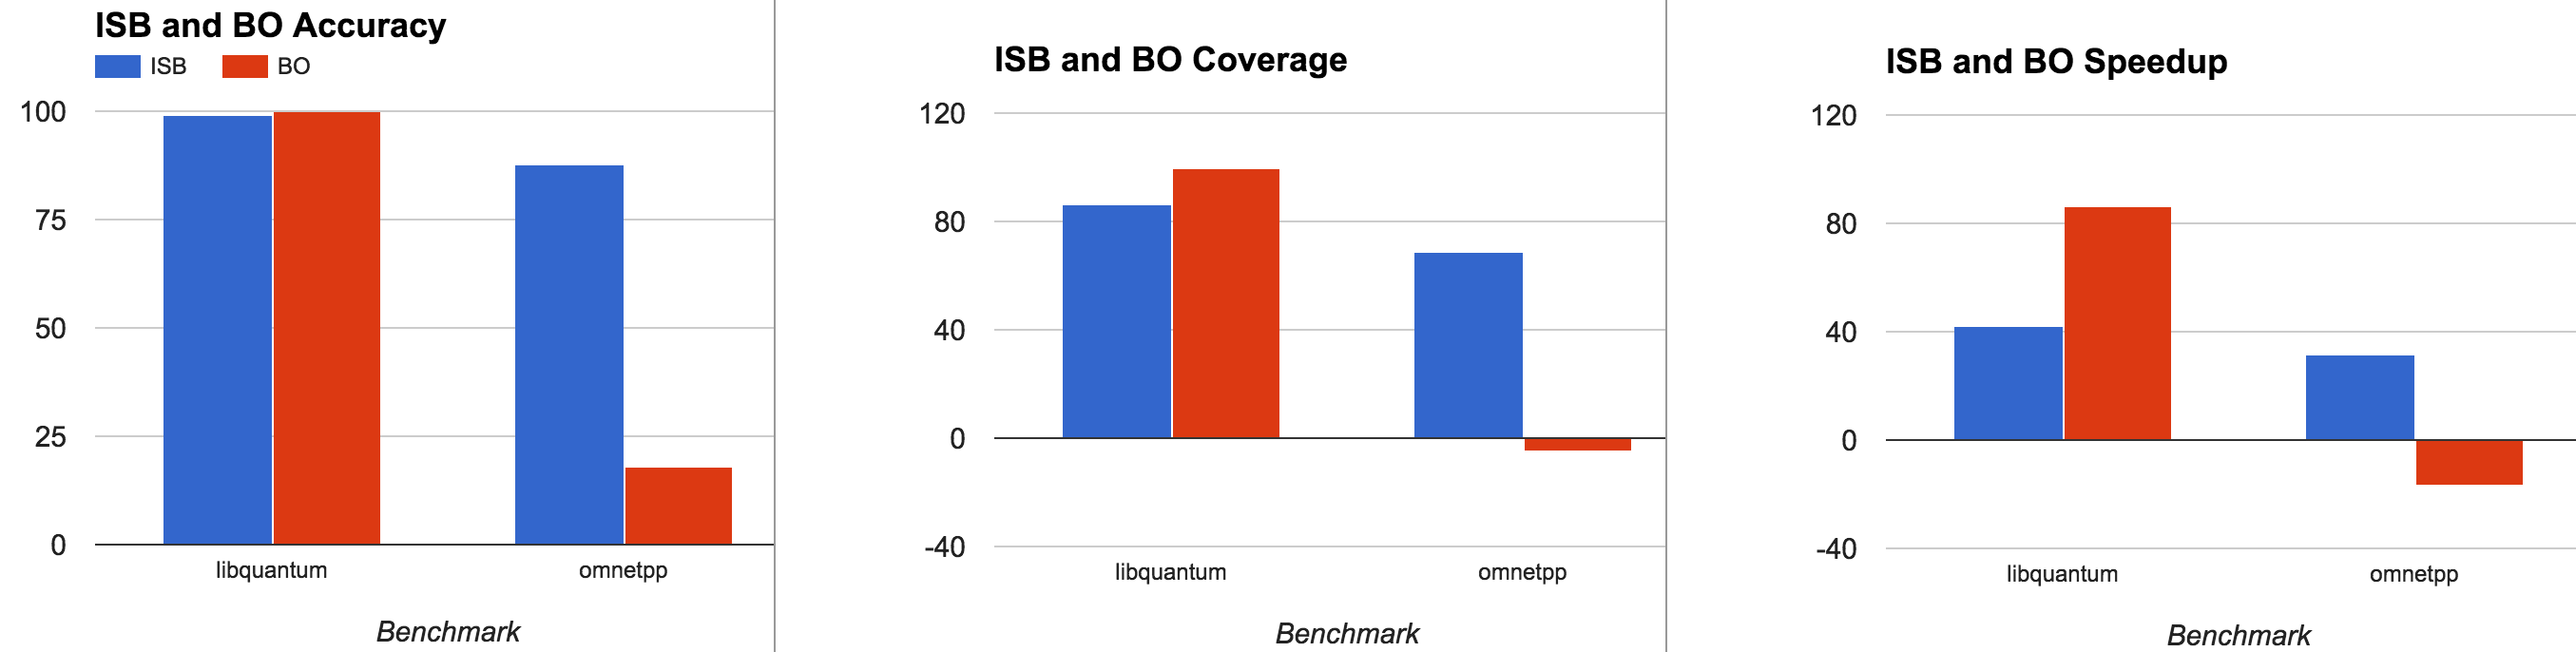
\includegraphics[width=1.0\textwidth]{images/isbvsbo.png}
	  \caption{\emph{ISB} and \emph{BO} performance comparision}
	  \label{fig:regVsirreg}
  \end{figure}


  \subsection{Naive Hybrid Prefetcher Vs. \emph{BO}\&\emph{ISB}}
  \label{sec:naivehy}
  One may ask a question after reading Section \ref{sec:irrVsre}: then why not issue prefetches from both prefetchers? We call hybrid prefetcher with this behavior \emph{Naive Hybrid Prefetcher, or NHP}.
  \begin{figure}[ht!]
	  \centering
	  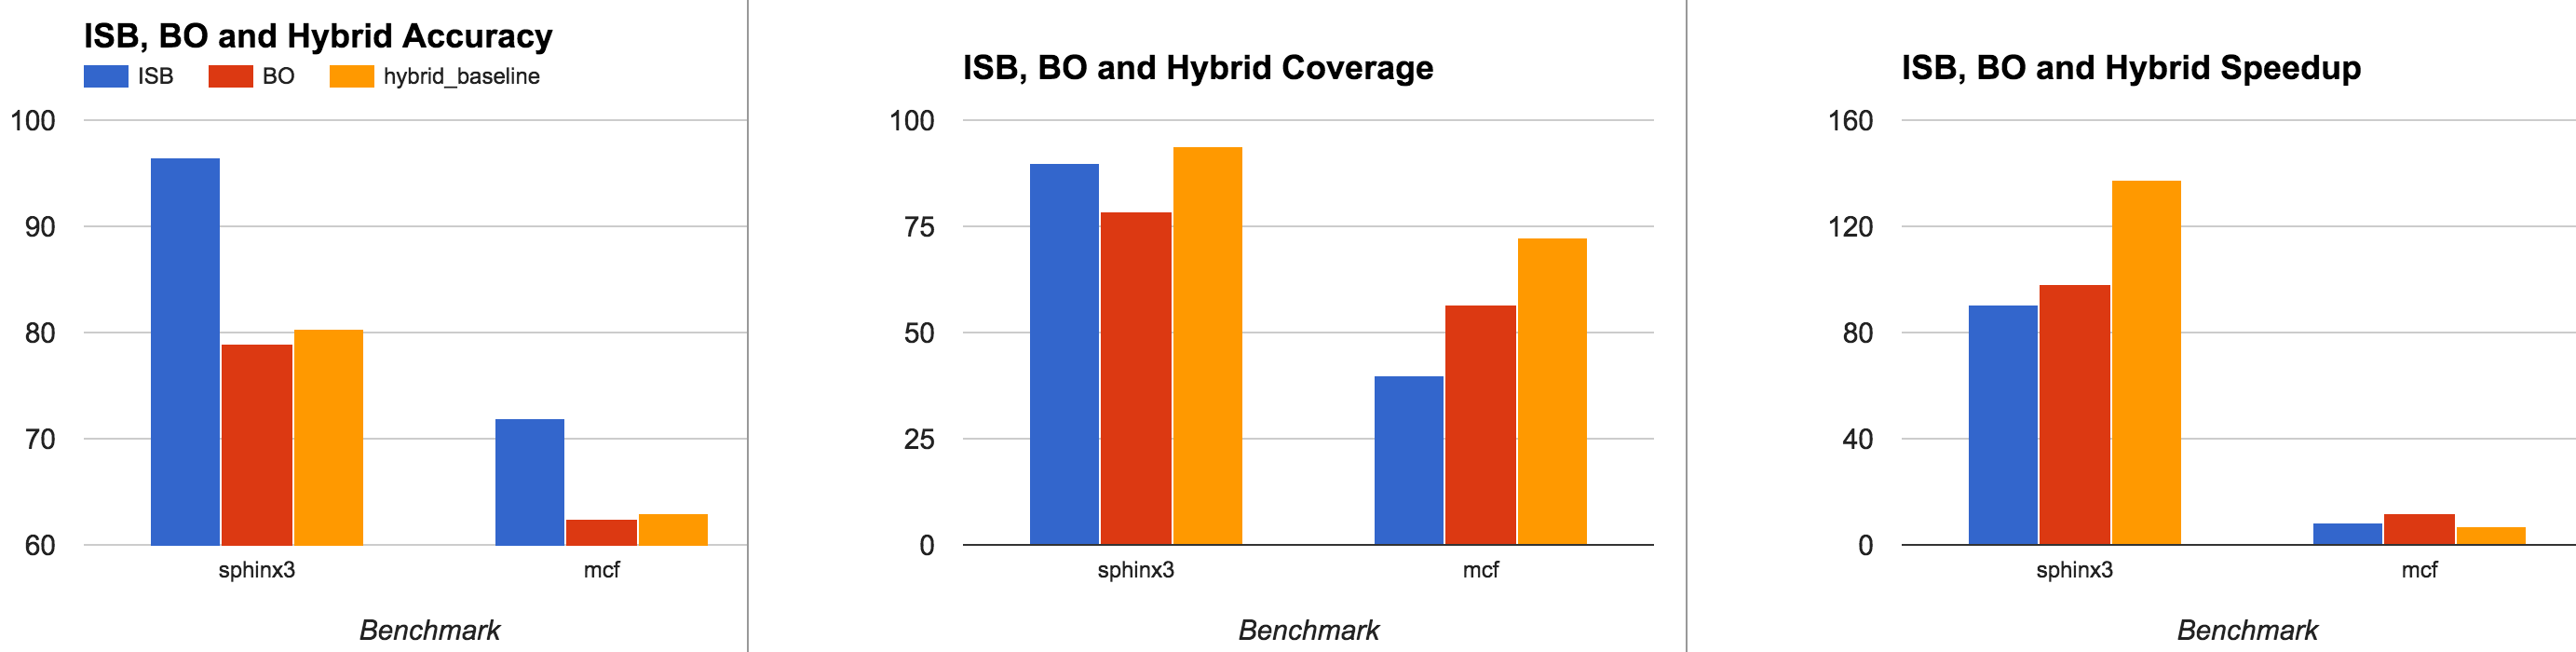
\includegraphics[width=1.0\textwidth]{images/hybridVssingle.png}
	  \caption{\emph{Naive Hybrid} and \emph{ISB, BO} performance comparision}
	  \label{fig:hybridVssingle}
  \end{figure}


  Well, it works when resource is rich enough, such as huge cache, huge memory bandwidth and so on. If these are limited, \emph{NHP} may cause huge memory pressure and cache pollution due to large number of inaccurate prefetches. In Fig.\ref{fig:hybridVssingle}, we give an example when \emph{NHP} works and when it doesn't. 
 Benchmark \emph{sphinx3} is not memory intensive. The figure shows that the accuracy of \emph{ISB} is much higher than \emph{NHP}'s while \emph{NHP}'s coverage is a little bit higher. This means that \emph{NHP} issued much more useless prefetches to the memory, to achieve a little bit higher coverage. Because the benchmark is not memory intensive, the many useless prefetches don't cost much overhead. \emph{NHP}'s speed is still much better than \emph{ISB}'s. 
 On the other hand, for memory intensive benchmark \emph{mcf}, \emph{ISB} also has higher accuracy and lower coverage. However, this time, \emph{NHP}'s speedup is lower than \emph{ISB}'s. The possible contention reasons that a \emph{NHP} results in poor performance are listed below.


  \begin{itemize}
    \item Memory bandwidth is limited
    \item Memory request buffer size is limited
    \item Cache size is limited
    \item Cache pollution
  \end{itemize}

  \subsection{Related Work}
  \label{sec:PrevSol}
  Gendler et al.\cite{gendlerpaper} proposed a method to combine multiple prefetchers.
  They calculate the accuracy of every prefetcher in the last N prefetched addresses and only turn on the most accurate one.
  This scheme doesn't take coverage into account and may result in bad choice: a high-accurate low-coverage prefetcher is preferred to a medium-high-accurate high coverage one.
  If the contention of resources is not an issue, the better choice is obviously the latter one. \par
  Ebrahimi et al.\cite{yalepaper} used an interval-based sampling and throttling method to control the aggressiveness of two prefetchers.
  In each interval, they sample the number of total prefetches, hits in prefetches and total misses to calculate the accuracy and coverage of each prefetcher.
  They combine the current statistics and historical statistics, and use the combination as the performance feedback of two prefetchers.
  Finally they build a heuristics to coordinate and throttle the prefetchers in the next interval.



\subsection{Our Scheme: PC Localization}
  \label{sec:goal}
  Our design of hybrid prefetcher should do prefetching smartly. Idealy, if our hybrid prefetcher can utilize \emph{BO} and \emph{ISB}'s advantage well while avoiding the influence of their disadvantages, the hybrid prefetcher should enjoy better accuracy, coverage and speedup. \par
  PC localization has been demonstrated as a useful technique in prefetching.\cite{isbpaper, ghbpaper, shippaper}. In this project we use PC as our feature to localize prefetchers. The intuition of PC localization is that PC is biased to regular patterns or irregular patterns.
  Some PCs traverse an array with a fixed stride so it would always load regular streams. Some PCs scan a linked list or a graph, so it will always load irregular streams.
  During the execution, if our hybrid prefetching system can identify the preference of each PC and control the prefetching degree of both prefetchers, we can make accurate prefetches and avoid useless prefetches. \par
